% Verified against ErrorTransitionEvaluator.createTransition and
% run-metrics-calculator.ts:getErrorResponseCategory.
\documentclass[11pt,tikz,border=7pt]{standalone}
\usepackage{fontspec}
\setmainfont{texgyreheros-regular.otf}[BoldFont=texgyreheros-bold.otf]
\usetikzlibrary{arrows.meta}
\definecolor{accent}{HTML}{32658A}
\hyphenpenalty=10000
\begin{document}
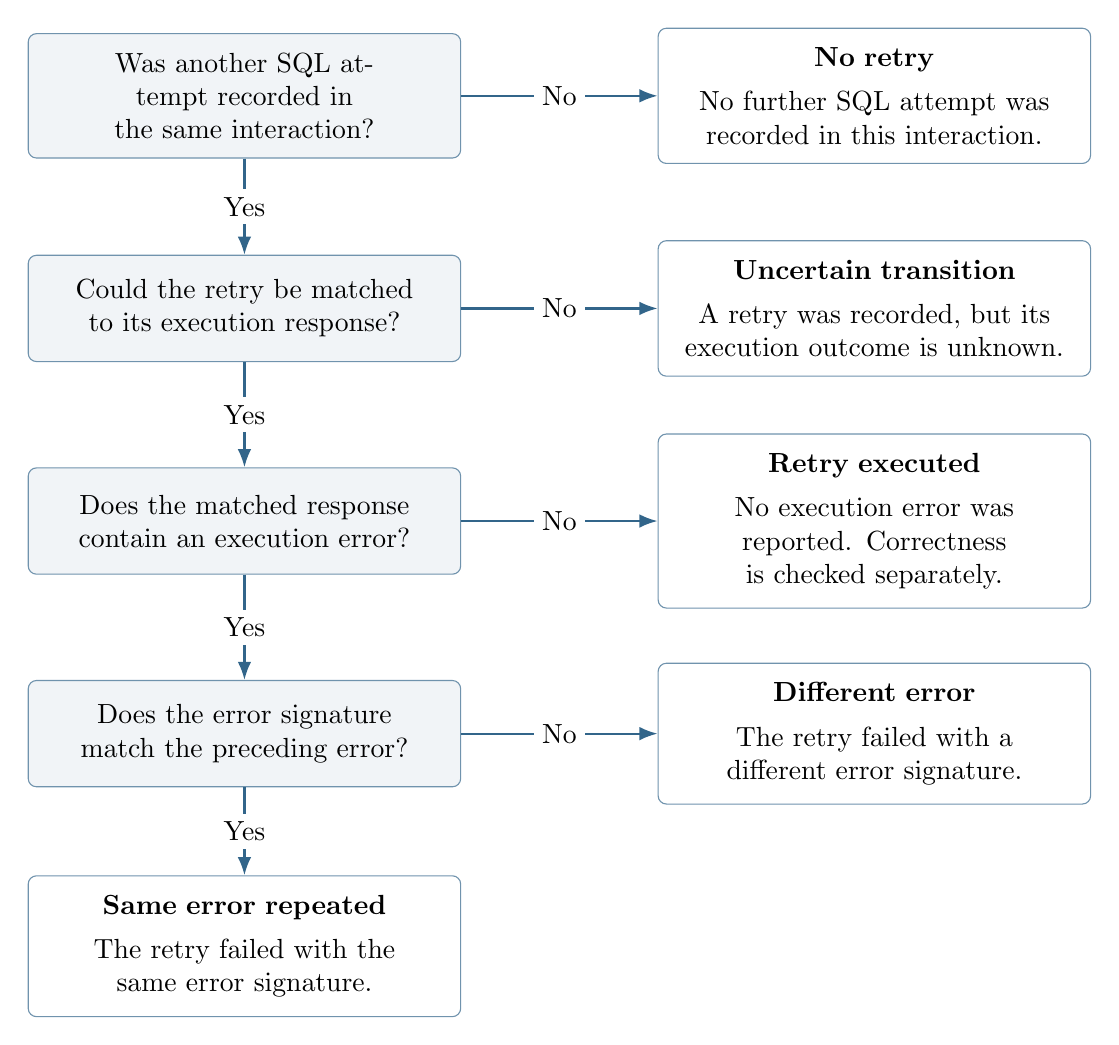
\begin{tikzpicture}[
  font=\normalsize,
  box/.style={draw=accent!70,rounded corners=3pt,align=center,
    inner sep=7pt,text width=5cm,minimum height=1.35cm},
  question/.style={box,fill=accent!7},
  result/.style={box,fill=white},
  flow/.style={-{Latex[length=2.3mm]},draw=accent,line width=.8pt},
  tag/.style={fill=white,inner sep=3pt,font=\normalsize}
]
\node[question] (retry) at (0,0)
  {Was another SQL attempt recorded in the same interaction?};
\node[result] (none) at (8,0)
  {\textbf{No retry}\\[4pt]No further SQL attempt was recorded in this interaction.};
\node[question] (matched) at (0,-2.7)
  {Could the retry be matched to its execution response?};
\node[result] (uncertain) at (8,-2.7)
  {\textbf{Uncertain transition}\\[4pt]A retry was recorded, but its execution outcome is unknown.};
\node[question] (error) at (0,-5.4)
  {Does the matched response contain an execution error?};
\node[result] (executed) at (8,-5.4)
  {\textbf{Retry executed}\\[4pt]No execution error was reported. Correctness is checked separately.};
\node[question] (same) at (0,-8.1)
  {Does the error signature match the preceding error?};
\node[result] (different) at (8,-8.1)
  {\textbf{Different error}\\[4pt]The retry failed with a different error signature.};
\node[result] (repeated) at (0,-10.8)
  {\textbf{Same error repeated}\\[4pt]The retry failed with the same error signature.};
\foreach \from/\to in {retry/matched,matched/error,error/same,same/repeated}
  \draw[flow] (\from)--node[tag]{Yes}(\to);
\foreach \from/\to in {retry/none,matched/uncertain,error/executed,same/different}
  \draw[flow] (\from)--node[tag]{No}(\to);
\end{tikzpicture}
\end{document}
